\subsection{Introduction}

\begin{frame}[containsverbatim]
	\frametitle{What will we learn today ?}	
	\begin{itemize}
		\item {Advanced \verb+MPI_Types+, MPI communicators and groups (MPI 1.0)}
		\item {Persistent communications (MPI 2.0)}
		\item {One-sided communications (RMA) (MPI 2.0 and MPI 3.0)}
		\item {Dynamic process management (MPI 2.0)}
		\item {Parallel I/O (MPI 2.0)}
		\item {Non-blocking collectives (MPI 3.0)}
	\end{itemize}
\end{frame}


\subsection{Advanced MPI$\_$Types}


\begin{frame}[containsverbatim]
\frametitle{Basic MPI datatypes (C)}

\begin{center}
\begin{tabular}{ | l | l | }
	\hline 
	\textbf{C datatype} & \textbf{MPI datatype} \\
	\hline 
	\hline 
	signed char & MPI$\_$CHAR\\
	signed short int & MPI$\_$SHORT\\
	signed int & MPI$\_$INT \\
	signed long int & MPI$\_$LONG \\
	unsigned char & MPI$\_$UNSIGNED$\_$CHAR\\
	unsigned short int & MPI$\_$UNSIGNED$\_$SHORT\\
	unsigned long int & MPI$\_$UNSIGNED$\_$LONG\\
	unsigned int & MPI$\_$UNSIGNED\\
	float & MPI$\_$FLOAT\\
	double & MPI$\_$DOUBLE\\
	long double & MPI$\_$LONG$\_$DOUBLE\\
	\hline 
 \end{tabular}
\end{center}
\end{frame}


\begin{frame}[containsverbatim]
\frametitle{Basic MPI datatypes (FORTRAN)}

\begin{center}
\begin{tabular}{ | l | l | }
	\hline 
	\textbf{FORTRAN datatype} & \textbf{MPI datatype} \\
	\hline 
	\hline 
	INTEGER & MPI$\_$INTEGER\\
	REAL & MPI$\_$REAL\\
	REAL*8 & MPI$\_$REAL8\\
	DOUBLE PRECISION & MPI$\_$DOUBLE$\_$PRECISION\\
	COMPLEX & MPI$\_$COMPLEX\\
	LOGICAL & MPI$\_$LOGICAL\\
	CHARACTER & MPI$\_$CHARACTER \\
	\hline 
 \end{tabular}
\end{center}
\end{frame}

\begin{frame}[containsverbatim]
\frametitle{Derived MPI datatypes}

OK. That is perfect when all the data are of the same type (integers, floats, characters, etc..). But how to send a structure using MPI ?

\begin{lstlisting}[language=C,frame=lines]
struct { 
   int x; int y;
   double vx; double vy;
   float mass;
} particle;
particle p = {1,2,0.3,0.4,1.0};
MPI_Send(p, ...);
\end{lstlisting}
\end{frame}


\begin{frame}[containsverbatim]
\frametitle{Derived MPI datatypes}
\begin{itemize}
	\item Definition of \textbf{new} datatypes by grouping basic MPI datatypes
	\item It is possible to group \begin{itemize} \item data from different types \item group non-contiguous data \end{itemize}
	\item A derived datatype is defined in three steps : \begin{itemize} \item construct the type \item commit it to the system \item free it \end{itemize}
\end{itemize}

\end{frame}



\begin{frame}[containsverbatim]
\frametitle{Derived MPI datatypes}	
\begin{itemize}
	\item \verb+MPI_Type_contiguous+ Produces a new data type by making copies of an existing data type. 
	\item \verb+MPI_Type_vector+, Similar to contiguous, but allows for regular gaps (stride) in the displacements
	\item \verb+MPI_Type_indexed+, An array of displacements of the input data type is provided as the map for the new data type.
	\item \verb+MPI_Type_create_struct+ The new data type is formed according to completely defined map of the component data types. 
	\item \verb+MPI_Type_extent+ Returns the size in bytes of the specified data type.
	\item \verb+MPI_Type_commit+ Commits new datatype to the system. 
	\item \verb+MPI_Type_free+ Deallocates the specified datatype object.
\end{itemize}

\end{frame}

\begin{frame}[containsverbatim]
\frametitle{MPI$\_$Type$\_$struct example}	

\begin{lstlisting}[language=C,frame=lines,basicstyle=\footnotesize]
struct foo { int a; char b; } f ; f.a = 1; f.b = 'z';
int blen[2];
MPI_Aint displs[2];
MPI_Datatype oldtypes[2];
MPI_Datatype newtype;

MPI_Aint zero_address, first_address, second_address;
MPI_Get_address(&f, &zero_address);
MPI_Get_address(&f.a, &first_address);
MPI_Get_address(&f.b, &second_address);
blen[0] = 1; displs[0] = MPI_Aint_diff(first_address, zero_address);
oldtypes[0] = MPI_INT; oldtypes[1] = MPI_CHAR;
blen[1] = 1; displs[1] = MPI_Aint_diff(second_address, zero_address);
MPI_Type_create_struct( 2, blen, displs, oldtypes, &newtype );
MPI_Type_commit(&newtype);

MPI_Send(&f, 1, newtype, 0, 100, MPI_COMM_WORLD );
MPI_Type_free( &newtype );
\end{lstlisting}
The MPI datatype \texttt{newtype} is a structure that contains \texttt{\{f\}}



%\begin{frame}[containsverbatim]
%\frametitle{MPI$\_$Type$\_$struct example}	

%\begin{lstlisting}[language=C,frame=lines]
%struct { int a; char b; } foo;
%foo f = {1,'z'};
%MPI_Aint zero_address, first_address, second_address;
%MPI_Get_address(&foo, &zero_address);
%MPI_Get_address(&foo.a, &first_address);
%MPI_Get_address(&foo.b, &second_address);
%MPI_Datatype newtype;
%MPI_Aint displs[2];
%blen[0] = 1; indices[0] = MPI_Aint_diff(first_address, zero_address);
%oldtypes[0] = MPI_INT; oldtypes[1] = MPI_CHAR;
%blen[1] = 1; indices[1] = MPI_Aint_diff(second_address, zero_address); 
%MPI_Type_create_struct( 2, blen, indices, oldtypes, &newtype );
%MPI_Type_Commit(&newtype);
%MPI_Send(&f, 1, newtype, 0, 100, MPI_COMM_WORLD );
%MPI_Type_free( &newtype );
%\end{lstlisting}
%The MPI datatype \texttt{newtype} is a structure that contains \texttt{\{foo\}}



% =============================================================
% EXOS 2018 avec correction
% =============================================================
%  MPI_Aint zero_address, first_address, second_address;                            
%  MPI_Get_address(&send, &zero_address);                                            
%  MPI_Get_address(&send.sum, &first_address);                                      
%  MPI_Get_address(&send.rank, &second_address);                                    
%                                                                                    
%  MPI_Aint displs[2];                                                              
%  displs[0] = MPI_Aint_diff(first_address, zero_address);;                          
%  displs[1] = MPI_Aint_diff(second_address, zero_address);                        
%                                                                                    
%  MPI_Datatype types[2] = {MPI_DOUBLE, MPI_INT};                                    
%  MPI_Datatype sum_t;                                                              
%  MPI_Type_create_struct(2, blk_length, displs, types, &sum_t);                    
%  MPI_Type_commit(&sum_t)
% =============================================================


%\begin{lstlisting}[language=C,frame=lines]
%int blocklens[7];
%MPI_Datatype myparticle;
%MPI_Datatype old_types[5];
%old_types[0] = MPI_INT; old_types[1] = MPI_INT;
%old_types[2] = MPI_DOUBLE; old_types[3] = MPI_DOUBLE;
%old_types[4] = MPI_FLOAT;
%blocklens[0] = 1; blocklens[1] = 1; blocklens[2] = 1;
%blocklens[3] = 1; blocklens[4] = 1;
%MPI_Address( &particle.x, &indices[0] ); MPI_Address( &particle.y, &indices[1] );
%MPI_Address( &particle.vx, &indices[2] ); MPI_Address( &particle.vy, &indices[3] );
%MPI_Address( &particle.mass, &indices[4] );
%MPI_Type_struct( 5, blocklens, indices, old_types, &myparticle );
%MPI_Send( &p, 1, myparticle, 0, 100, MPI_COMM_WORLD );
%MPI_Type_free( &myparticle );
%\end{lstlisting}

\end{frame}

\begin{frame}[containsverbatim]
\frametitle{Extents}	
FIXME : MPI_Type_create_resized()
\end{frame}





\begin{frame}[containsverbatim]
\frametitle{Pack/Unpack data}	
\begin{itemize}
	\item { Instead of creating a new datatype, it is possible to pack and unpack data of different types }
	\item { Less good than MPI derived datatypes in terms of memory usage and performance }
	\item { ``just like a streaming'' }
	\item { \verb+int MPI_Pack(const void *inbuf, int incount, +\\\verb+MPI_Datatype datatype, void *outbuf, int outsize,+\\\verb+ int *position, MPI_Comm comm)+}
	\item { \verb+int MPI_Unpack(const void *inbuf, int insize,+\\\verb+ int *position, void *outbuf, int outcount, +\\\verb+MPI_Datatype datatype, MPI_Comm comm)+}
\end{itemize}
\end{frame}


\begin{frame}[containsverbatim]
\frametitle{Pack/Unpack data}	
\begin{lstlisting}[language=C,frame=lines]
int x; float a, int position=0;
char buffer[100];
if (myrank==0)
   MPI_Pack(&a, 1, MPI_FLOAT, buffer, 100, &position, MPI_COMM_WORLD)
   MPI_Pack(&x, 1, MPI_INT, buffer, 100, &position, MPI_COMM_WORLD)
   MPI_Send(buffer, 100, MPI_PACKED, 1, 999, MPI_COMM_WORLD);
}else if (myrank==1) {
   MPI_Recv(buffer, 100, MPI_PACKED, 0, 999, MPI_COMM_WORLD, status)
   MPI_Unpack(buffer, 100, &position, &a, 1, MPI_FLOAT, MPI_COMM_WORLD);
   MPI_Unpack(buffer, 100, &position, &x, 1, MPI_INT, MPI_COMM_WORLD);
}
\end{lstlisting}
\end{frame}


\subsection{MPI communicators and groups}



\begin{frame}[containsverbatim]
\frametitle{MPI Groups and Communicators}	
MPI Groups :
\begin{itemize}
	\item {ordered set of processes}
	\item {each process has an unique ID (rank within the group) and can belong to several different groups}
	\item {a group can be used to create a new communicator}
\end{itemize}
MPI Communicators :
\begin{itemize}
	\item {A group of processes}
	\item {encapsulate the communications between the belonging processes}
	\item {An MPI communication can take place only with a communicator (not a group)}
\end{itemize}
\end{frame}


\begin{frame}[containsverbatim]
\frametitle{MPI Groups and Communicators}	
\begin{center}
% Slide 194
\begin{tikzpicture}[scale=0.7, every node/.style={scale=0.8}]
\node[label = {above:\texttt{MPI\_COMM\_WORLD}}, ellipse, draw, minimum height = 3cm, minimum width = 6cm, dashed, outer sep = 3pt] (W) at (0,0) {};

\node[circle, draw, inner sep = 3pt] at (-2, 0) {2};
\node[circle, draw, inner sep = 3pt] at (-1.3, -0.3) {1};
\node[circle, draw, inner sep = 3pt] at (-1, 0.4) {6};
\node[circle, draw, inner sep = 3pt] at (-0.2, 0) {0};
\node[circle, draw, inner sep = 3pt] at (0.4, 0.5) {7};
\node[circle, draw, inner sep = 3pt] at (0.6, -0.5) {3};
\node[circle, draw, inner sep = 3pt] at (1.3, 0) {5};
\node[circle, draw, inner sep = 3pt] at (2.3, 0) {4};

\node[ellipse, label = {left:{Group 1}}, minimum height = 2cm, minimum width = 3cm] (G1) at (-3, -3) {};
\node[circle, draw, inner sep = 3pt] at (-3.4, -2.6) {1};
\node[circle, draw, inner sep = 3pt] at (-2.6, -2.6) {3};
\node[circle, draw, inner sep = 3pt] at (-3.8, -3.3) {2};
\node[circle, draw, inner sep = 3pt] at (-3, -3.3) {0};
\node[circle, draw, inner sep = 3pt] at (-2.2, -3.3) {4};

\node[ellipse, label = {right:{Group 2}}, minimum height = 2cm, minimum width = 1.5cm] (G2) at (3, -3) {};
\node[circle, draw, inner sep = 3pt] at (3.2, -3.4) {7};
\node[circle, draw, inner sep = 3pt] at (3.2, -2.6) {6};
\node[circle, draw, inner sep = 3pt] at (2.5, -3) {5};

\draw[->] (W) -- (G1);
\draw[->] (W) -- (G2);

\begin{scope}[yshift = -2.6cm]
\node[draw, blue2, outer sep = 3pt, dashed, ellipse, label = {below:{MPI Communicator (Group1)}}, minimum height = 2cm, minimum width = 3cm] (GC1) at (-3, -3) {};
\node[circle, draw, inner sep = 3pt] at (-3.4, -2.6) {1};
\node[circle, draw, inner sep = 3pt] at (-2.6, -2.6) {3};
\node[circle, draw, inner sep = 3pt] at (-3.8, -3.3) {2};
\node[circle, draw, inner sep = 3pt] at (-3, -3.3) {0};
\node[circle, draw, inner sep = 3pt] at (-2.2, -3.3) {4};

\node[draw, blue2, outer sep = 3pt, dashed, ellipse, label = {below:{MPI Communicator (Group2)}}, minimum height = 2cm, minimum width = 3cm] (GC2) at (3, -3) {};
\node[circle, draw, inner sep = 3pt] at (3.2, -3.4) {7};
\node[circle, draw, inner sep = 3pt] at (3.2, -2.6) {6};
\node[circle, draw, inner sep = 3pt] at (2.5, -3) {5};
\end{scope}

\draw[->] (G1) -- (GC1);
\draw[->] (G2) -- (GC2);

\end{tikzpicture}

\end{center}
\end{frame}



\begin{frame}[containsverbatim]
\frametitle{Create a new communicator}	

%\begin{lstlisting}[language=C,frame=lines]
%main(int argc, char *argv[])  {
% int myrank, new_rank, sendbuf, recvbuf, mysize,
% MPI_Group  old_grp, new_grp;
% MPI_Comm   new_comm;
% MPI_Init(&argc,&argv);
% MPI_Comm_rank(MPI_COMM_WORLD, &rank);
% MPI_Comm_size(MPI_COMM_WORLD, &size);
% MPI_Comm_group(MPI_COMM_WORLD, &old_group);
% if (rank < NPROCS/2) {
%  MPI_Group_incl(old_grp, size/2, ranks1, &new_grp);
% } else {
%  MPI_Group_incl(old_grp, size/2, ranks2, &new_grp);
% }
% MPI_Comm_create(MPI_COMM_WORLD,new_group,&new_comm);
% MPI_Group_rank (new_group, &new_rank);
% printf("rank= %d newrank= %d recvbuf= %d\n",rank,new_rank,recvbuf);
% MPI_Finalize();
%}
%\end{lstlisting}


\begin{lstlisting}[language=C,frame=lines]
 MPI_Init(&argc,&argv);
 MPI_Comm_rank(MPI_COMM_WORLD, &rank);
 MPI_Comm_size(MPI_COMM_WORLD, &size);
 MPI_Comm_group(MPI_COMM_WORLD, &old_g);
 int nbr_g1 = 5;
 ranks1 = (int*) malloc(nbr_g1*sizeof(int));
 ranks2 = (int*) malloc((size-nbr_g1)*sizeof(int));
 for (i=0;i<nbr_grp1;i++)  ranks1[i]=i;
 for (i=0;i<(size-nbr_g1);i++) ranks2[i]=size-i-1;
 if (rank < nbr_g1) {
  MPI_Group_incl(old_g,nbr_g1,ranks1,&new_g);
 } else {
  MPI_Group_incl(old_g,(size-nbr_g1),ranks2,&new_g);
 } 
 MPI_Comm_create(MPI_COMM_WORLD,new_g,&new_comm);
 MPI_Group_rank (new_g, &new_rank);
 printf("rank %d grprank is %d \n",rank,new_rank);
 MPI_Finalize();
\end{lstlisting}


%\begin{lstlisting}[language=C,frame=lines]
% MPI_Group  old_grp, new_grp;
% MPI_Comm   new_comm;
% MPI_Init(&argc,&argv);
% MPI_Comm_rank(MPI_COMM_WORLD, &rank);
% MPI_Comm_size(MPI_COMM_WORLD, &size);
% MPI_Comm_group(MPI_COMM_WORLD, &old_group);
% if (rank < NPROCS/2) {
%  MPI_Group_incl(old_grp, size/2, ranks1, &new_grp);
% } else {
%  MPI_Group_incl(old_grp, size/2, ranks2, &new_grp);
% }
% MPI_Comm_create(MPI_COMM_WORLD,new_group,&new_comm);
% MPI_Group_rank (new_group, &new_rank);
% printf("rank= %d newrank= %d recvbuf= %d\n",rank,new_rank,recvbuf);
% MPI_Finalize();
%\end{lstlisting}


\end{frame}


\subsection{Persistent communications}

\begin{frame}[containsverbatim]
\frametitle{Persistent communications}
\begin{itemize}
	\item {when a same communication is repeated within a loop (e.g. exchanging neighbors in 2D Poisson) }
	\item {Improvement can be done using a persistent communication}
	\item {Using a \verb+MPI_Request+ to initiate and complete a communication}
	\item {\verb+MPI_Send_Init()+ : creates a persistent communication request for a standard mode send operation }
	\item {\verb+MPI_Bsend_Init()+ : creates a persistent communication request for a bufferd mode send operation}
	\item {\verb+MPI_Ssend_Init()+ : creates a persistent communication object for a synchronous mode send operation}
	\item {\verb+MPI_Rsend_Init()+ : creates a persistent communication object for a ready mode send operation}
	\item {\verb+MPI_Recv_Init()+ : creates a persistent communication request for a receive operation.}
\end{itemize}
\end{frame}


\begin{frame}[containsverbatim]
\frametitle{Persistent communications example}	

\begin{lstlisting}[language=C,frame=lines,basicstyle=\footnotesize]
   MPI_Request recvreq;
   MPI_Request sendreq;

   MPI_Recv_init (buffer, N, MPI_FLOAT, rank-1, tag_check_infos, MPI_COMM_WORLD, &recvreq);
   MPI_Send_init (buffer, N, MPI_FLOAT, rank+1, tag_check_infos, MPI_COMM_WORLD, &sendreq);

/* ... copy stuff into buffer ... */

   MPI_Start(&sendreq);         
   MPI_Start(&recvreq);         
   MPI_Wait(&sendreq, &status); 
   MPI_Wait(&recvreq, &status); 

   MPI_Request_free( &recvreq );
   MPI_Request_free( &sendreq );
\end{lstlisting}
\end{frame}




\subsection{Remote Memory Access (One-sided communications)}

\begin{frame}[containsverbatim]
\frametitle{One-sided communication}
\begin{itemize}
	\item {A MPI process can access another MPI process's memory space directly (RMA)}
	\item {No explicit coordination between both processes}
	\item {explicit transfer, explicit synchronization}
	\item {Better performance}
\end{itemize}
\end{frame}

\begin{frame}[containsverbatim]
\frametitle{One-sided communication}
Initialization/Free (of the \textit{window} = window in memory)
\begin{itemize}
	\item {\verb+MPI_Alloc_Mem()+, \verb+MPI_Free_Mem()+}
	\item {\verb+MPI_Win_Create()+, \verb+MPI_Win_Free()+}
\end{itemize}
Remote memory access
\begin{itemize}
	\item {\verb+MPI_Put()+ (like send)}
	\item {\verb+MPI_Get()+ (like recv)}
	\item {\verb+MPI_Accumulate()+ (like reduce)}
\end{itemize}
Synchronization
\begin{itemize}
	\item {\verb+MPI_Win_Fence()+}
	\item {\verb+MPI_Win_Post()+, \verb+MPI_Win_Start()+, \verb+MPI_Win_Complete()+, \verb+MPI_Win_Wait()+}
	\item {\verb+MPI_Win_Lock()+, \verb+MPI_Win_Unlock()+}
\end{itemize}

\end{frame}

\begin{frame}[containsverbatim]
\frametitle{Memory allocation}
\begin{itemize}
	\item {allocate \verb+size+ of memory segments in bytes}
	\item {\verb+info+ can be used to provide directives that control the desired location of the allocated memory}
	\item {\verb+*baseptr+ is the pointer to the beginning of the memory segment}
\end{itemize}

\begin{lstlisting}[language=C,frame=lines]
int MPI_Alloc_mem(MPI_Aint size, MPI_Info info, void *baseptr)
\end{lstlisting}

\end{frame}



\begin{frame}[containsverbatim]
\frametitle{Memory \texttt{window} creation}
\begin{itemize}
	\item {A \verb+MPI_Win+ is an opaque object which can be reused to perform one-sided communication}
	\item {A \verb+window+ is a specified region in memory that can be accessed by another process}
\end{itemize}

\begin{lstlisting}[language=C,frame=lines]
int MPI_Win_create(void *base, MPI_Aint size, int disp_unit, MPI_Info info, MPI_Comm comm, MPI_Win *win)
\end{lstlisting}

where \verb+base+ is the initial address of the region, of \verb+size+ length of size \verb+disp_unit+ in bytes.

\end{frame}

\begin{frame}[containsverbatim]
\frametitle{\texttt{Put}/\texttt{Get} within the \texttt{window}}
\begin{itemize}
	\item {close to an \verb+MPI_Send+ call with 
		\begin{itemize}
			\item {\textit{what to send} : \verb+origin_addr+ start of the buffer of size \verb+origin_count+ of type \verb+origin_datatype+}
			\item {\textit{to which process} : \verb+target_rank+ at the place \verb+target_count+ of type \verb+target_datatype+}
			\item {\textit{in which context} : within the window \verb+win+}
		\end{itemize}
	}
%	\item {}
\end{itemize}

\begin{lstlisting}[language=C,frame=lines]
int MPI_Put(const void *origin_addr, int origin_count, MPI_Datatype origin_datatype, int target_rank, MPI_Aint target_disp, int target_count, MPI_Datatype target_datatype, MPI_Win win)
\end{lstlisting}

\begin{lstlisting}[language=C,frame=lines]
int MPI_Get(void *origin_addr, int origin_count, MPI_Datatype origin_datatype, int target_rank, MPI_Aint target_disp, int target_count, MPI_Datatype target_datatype, MPI_Win win)
\end{lstlisting}


\end{frame}


\begin{frame}[containsverbatim]
\frametitle{One-sided communications example}

\begin{lstlisting}[language=C,frame=lines]
MPI_Win win;
int *mem;
float x = 1.0;
MPI_Alloc_mem(size * sizeof(int), MPI_INFO_NULL, &mem);
MPI_Win_create(mem, size * sizeof(int), sizeof(int), MPI_INFO_NULL, MPI_COMM_WORLD, &win);

// Write x at position 0 within process ranks's memory
MPI_Put(&x, 1, MPI_FLOAT, 0, rank, 1, MPI_INT, win);

MPI_Win_free(win);
MPI_Free_mem(mem);
\end{lstlisting}


\end{frame}


\begin{frame}[containsverbatim]
\frametitle{One-sided communications remarks}

\begin{itemize}
%	\item {Three primitives : Put (like a send), Get (like a recv) and accumulate (like a reduction)}
%	\item {synchronizations : fence / post-start-complete-wait / lock-unlock}
	\item {Pay attention to the memory coherence}
	\item {Can be dangerous : how a process knows if its data are in use/modified ?}
	\item {MPI-3 provides new features : \begin{itemize}
			\item cache-coherent windows,
			\item new primitives \verb+MPI_Get_accumulate()+, \verb+MPI_Fetch_and_op()+, \verb+MPI_Compare_and_swap+,
			\item requested-based primitives like \verb+MPI_R{put,get,accumulate,get_accumulate}+,
			\item ``all''-versions of the synchronization routines : \verb+MPI_Win_{un}lock_all+, \verb+MPI_Win_flush{_all}+, \verb+MPI_Win_flush_local{_all}+
			\end{itemize}
	}
%	\item {}
\end{itemize}
\end{frame}



\subsection{Dynamic Process Management}


\begin{frame}[containsverbatim]
\frametitle{Static model vs. Dynamic model}
MPI 1:
\begin{itemize}
	\item {Fixed number of MPI processes}
	\item {What happens if a process fail ? The entire job fails.}
	\item {impossible to ``inter-connect'' two independent MPI running jobs}
\end{itemize}
MPI 2 / MPI 3:
\begin{itemize}
	\item {support the creation of processes \textbf{on the fly} that can connect to existing running processes}
%	\item {\verb+MPI_Comm_spawn+ objects}
	\item {Concept of \textbf{intercommunicator} to handle the communications between parents and children}
	\item {Tricky !!}
\end{itemize}
\end{frame}


\begin{frame}[containsverbatim]
\frametitle{Master-Slave example (www.mpi-forum.org) -- Master}
\begin{lstlisting}[language=C,frame=lines]
int main(int argc, char *argv[]) { 
   int world_size, universe_size, *universe_sizep, flag; 
   MPI_Comm everyone;           /* intercommunicator */ 
   char worker_program[100]; 
   MPI_Init(&argc, &argv); 
   MPI_Comm_size(MPI_COMM_WORLD, &world_size); 
   MPI_Attr_get(MPI_COMM_WORLD, MPI_UNIVERSE_SIZE, &universe_sizep, &flag);  
   universe_size = *universe_sizep; 
   choose_worker_program(worker_program); 
   MPI_Comm_spawn(worker_program, MPI_ARGV_NULL, universe_size-1, MPI_INFO_NULL, 0, MPI_COMM_SELF, &everyone, MPI_ERRCODES_IGNORE); 
/ * Parallel code here.  */
   MPI_Finalize(); 
   return 0; }
\end{lstlisting}
\end{frame}


\begin{frame}[containsverbatim]
\frametitle{Master-Slave example (www.mpi-forum.org) -- Slave}
\begin{lstlisting}[language=C,frame=lines]
int main(int argc, char *argv[]) { 
   int size; 
   MPI_Comm parent; 
   MPI_Init(&argc, &argv); 
   MPI_Comm_get_parent(&parent); 
   if (parent == MPI_COMM_NULL) error("No parent!"); 
   MPI_Comm_remote_size(parent, &size); 
   if (size != 1) error("Something's wrong with the parent"); 
 
/ * Parallel code here.  */

   MPI_Finalize(); 
   return 0; 
} 
\end{lstlisting}
\end{frame}



\subsection{Parallel I/O with MPI}

\begin{frame}[containsverbatim]
\frametitle{Introducing remarks}
\begin{itemize}
	\item {I/O is often (if not always) the main bottleneck in a parallel application}
	\item {MPI provides a mechanism to read/write in parallel}
\end{itemize}

\begin{center}
% Slide 208
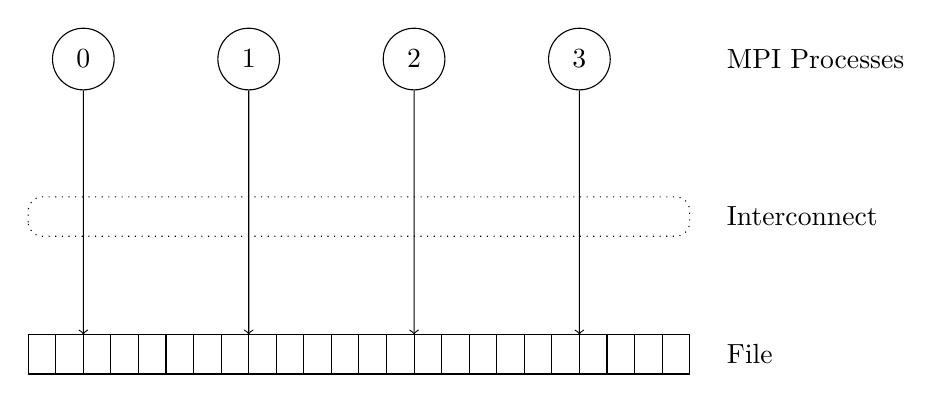
\begin{tikzpicture}[xscale = 0.7]

\draw[step = 0.5cm] (0,0) grid (12, 0.5);

\foreach \x[count = \i from 0] in {1, 4, ..., 10} {
	\node[circle, draw, inner sep = 5pt] (\i) at (\x, 4) {\i};
	\draw[->] (\i) -- (\x, 0.5);
}

\node[anchor = west] at (12.5, 4) {MPI Processes};
\node[anchor = west] at (12.5, 2) {Interconnect};
\node[anchor = west] at (12.5, 0.25) {File};

\draw[dotted, rounded corners = 5pt] (0,1.75) rectangle (12, 2.25);


\end{tikzpicture}

\end{center}
\end{frame}


\begin{frame}[containsverbatim]
\frametitle{Introducing remarks}
\begin{itemize}
	\item {MPI IO API works on your desktop/laptop}
	\item {Most of the large HPC systems have a \textbf{parallel file system} (like GPFS, Lustre, etc..)}
	\item {If the file is distributed smartly on a parallel file system : performance increases}
	\item {MPI IO offers a high-level API to access a distributed file (no needs to implement complexe POSIX calls)}
	\item {\textbf{does not work with ASCII files}}
	\item {Most of the standard file format support MPI IO (e.g. HDF5, NetCDF, etc..)}
\end{itemize}
\end{frame}


\begin{frame}[containsverbatim]
\frametitle{Poisson so far}
\begin{center}
% Slide 210
\begin{tikzpicture}[xscale = 0.8]


\foreach \x/\c[count = \i from 0] in {0/blue8, 3/blue4, 6/yellowbrown4, 9/yellowbrown2} {
	\node[outer sep = 3pt, fill = \c!40!white, circle, draw, inner sep = 5pt] (\i) at (\x, 4) {\i};
	\fill[\c!40!white] (\x, 0) rectangle (\x + 3, 0.5);
}

\draw[step = 0.5cm] (0,0) grid (12, 0.5);

\draw[->] (1) to[bend left] (0);
\draw[->] (2) to[bend left] (0);
\draw[->] (3) to[bend left] node[pos = 0.3, right, xshift = 0.5cm] {\texttt{MPI\_send(mypart, 0)}} (0);

\draw[->] (0.north east) to[out = 70, in = 110, looseness = 2] (0.north west);
\draw[->] (0) to[bend right] node[midway, right] {\texttt{Write()}} (-0.05, 0.55);
\end{tikzpicture}

\end{center}
\end{frame}

\begin{frame}[containsverbatim]
\frametitle{Poisson ideal}
\begin{center}
% Slide 210
\begin{tikzpicture}[xscale = 0.8]


\foreach \x/\c[count = \i from 0] in {0/blue8, 3/blue4, 6/yellowbrown4, 9/yellowbrown2} {
	\node[outer sep = 3pt, fill = \c!40!white, circle, draw, inner sep = 5pt] (\i) at (\x, 4) {\i};
	\fill[\c!40!white] (\x, 0) rectangle (\x + 3, 0.5);
	\draw[->] (\i) -- (\x, 0.55);
}

\node[anchor = west] at (9, 2) {\texttt{MPI\_File\_Write()}};

\draw[step = 0.5cm] (0,0) grid (12, 0.5);

\end{tikzpicture}

\end{center}
\end{frame}


\begin{frame}[containsverbatim]
\frametitle{Open/Close a file in parallel}
\begin{itemize}
	\item {\verb+comm+ : the communicator that contains the writing/reading MPI processes}
	\item {\verb+*filename+ : a file name}
	\item {\verb+amode+ : file access mode (Read only \verb+MPI_MODE_RDONLY+, read/write \verb+MPI_MODE_RDWR+, create \verb+MPI_MODE_CREATE+, etc..)}
	\item {\verb+info+ : file info object}
	\item {\verb+*fh+ : file handle}
\end{itemize}

\begin{lstlisting}[language=C,frame=lines]
int MPI_File_open(MPI_Comm comm, const char *filename, int amode, MPI_Info info, MPI_File *fh)
\end{lstlisting}

\begin{lstlisting}[language=C,frame=lines]
int MPI_File_close(MPI_File *fh)
\end{lstlisting}
\textbf{Collective calls !!}
\end{frame}


\begin{frame}[containsverbatim]
\frametitle{etype, offset and displacement}
\begin{itemize}
	\item {\textbf{etype} is the elementary type of the data of the parallel accessed file}
	\item {\textbf{offset} is a position in the file in term of multiple of etypes}
	\item {\textbf{displacement} of a position within the file is the number of bytes from the beginning of the file}
\end{itemize}
\begin{center}
% Slide 213
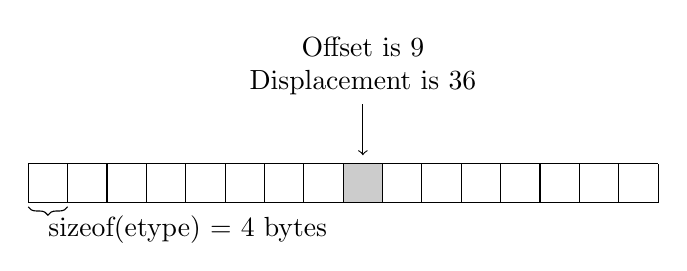
\begin{tikzpicture}
\draw[step = 0.5cm] (0,0) grid (8, 0.5);

\node[rectangle, draw, inner sep = 0.25cm, fill = gray!40!white, outer sep = 3pt] (R) at (4.25, 0.25) {};
\node[align = center, anchor = south] (W) at (4.25, 1.25) {Offset is 9 \\ Displacement is 36};

\draw[<-] (R) -- (W);

\draw[decorate,decoration={brace,amplitude=3pt, mirror}] (0, -0.05) -- (0.5, -0.05);
\node[anchor = north west, inner sep = 0pt] at (0.25, -0.15) {sizeof(etype) = 4 bytes};

\end{tikzpicture}

\end{center}
\end{frame}


\begin{frame}[containsverbatim]
\frametitle{Simple independent read/write}
\begin{itemize}
	\item {Can be used from a single (or group) of processes}
	\item {The \verb+offset+ must be specified in the \verb+*buf+ buffer}
	\item {\verb+count+ elements of type \verb+datatype+ are written}
\end{itemize}
\begin{lstlisting}[language=C,frame=lines]
int MPI_File_write_at(MPI_File fh, MPI_Offset offset, ROMIO_CONST void *buf, int count, MPI_Datatype datatype, MPI_Status *status)
\end{lstlisting}
\begin{lstlisting}[language=C,frame=lines]
int MPI_File_read_at(MPI_File fh, MPI_Offset offset, void *buf,int count, MPI_Datatype datatype, MPI_Status *status)
\end{lstlisting}
\end{frame}


\begin{frame}[containsverbatim]
\frametitle{\texttt{view} by each process}
\begin{itemize}
	\item {Initialy, each process view the file as a linear byte stream and each process views data in its own native representation}
	\item {this is changed using \verb+MPI_File_set_view+}
	\item {\verb+disp+ is the displacement (defines the beginning of the data of the file that belongs to the process) in bytes}
	\item {\verb+etype+ is the elementary type}
\end{itemize}
\begin{lstlisting}[language=C,frame=lines]
int MPI_File_set_view(MPI_File fh, MPI_Offset disp, MPI_Datatype etype, MPI_Datatype filetype, ROMIO_CONST char *datarep, MPI_Info info)
\end{lstlisting}
\begin{lstlisting}[language=C,frame=lines]
int MPI_File_get_view(MPI_File fh, MPI_Offset *disp, MPI_Datatype *etype, MPI_Datatype *filetype, char *datarep)
\end{lstlisting}
\end{frame}

\begin{frame}[containsverbatim]
\frametitle{Setting up a \texttt{view}}
\begin{center}
% Slide 216
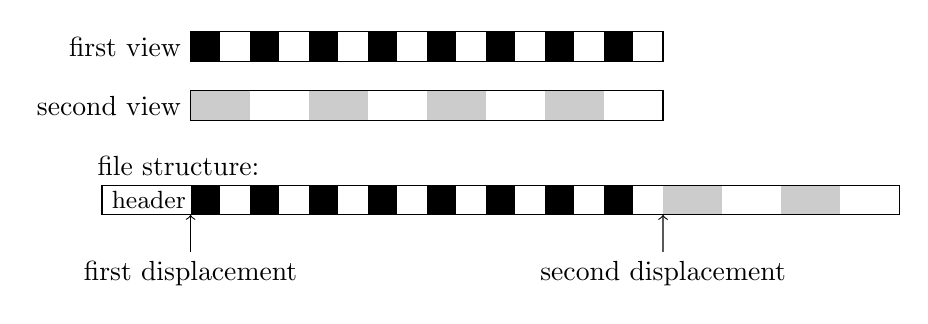
\begin{tikzpicture}[scale=0.75]

\node[anchor = east] at (0, 1.25) {first view};
\node[anchor = east] at (0, 0.25) {second view};

\foreach \x in {0, 1, 2, ..., 7.5}
	\fill[black] (\x, 1) rectangle (\x + 0.5, 1.5);

\foreach \x in {0, 2, ..., 7.5}
	\fill[gray!40!white] (\x, 0) rectangle (\x + 1, 0.5);

\draw (0, 1) rectangle (8, 1.5);
\draw (0, 0) rectangle (8, 0.5);

\begin{scope}[yshift = -1.6cm]
\node[anchor = south west, xshift = -0.18cm] at (-1.5, 0.5) {file structure:};

\node[anchor = west] at (-1.5, 0.25) {\small header};

\foreach \x in {0, 1, 2, ..., 7.5}
	\fill[black] (\x, 0) rectangle (\x + 0.5, 0.5);

\foreach \x in {0, 2, ..., 3.5}
	\fill[gray!40!white] (\x + 8, 0) rectangle (\x + 9, 0.5);

\draw (-1.5, 0) rectangle (12, 0.5);

\node (D1) at (0, -1) {first displacement};
\node (D2) at (8, -1) {second displacement};

\draw[->] (D1) -- (0,0);
\draw[->] (D2) -- (8,0);
\end{scope}

\end{tikzpicture}

\end{center}
(source : MPI 2.2 specifications)
\end{frame}

\begin{frame}[containsverbatim]
\frametitle{Simple independent read/write without offset}
\begin{itemize}
	\item {the \texttt{view} is specified prior to the call }
\end{itemize}
\begin{lstlisting}[language=C,frame=lines]
int MPI_File_write(MPI_File fh, ROMIO_CONST void *buf, int count, MPI_Datatype datatype, MPI_Status *status)
\end{lstlisting}
\begin{lstlisting}[language=C,frame=lines]
int MPI_File_read(MPI_File fh, void *buf, int count,MPI_Datatype datatype, MPI_Status *status)
\end{lstlisting}
\end{frame}


\begin{frame}[containsverbatim]
\frametitle{Collective read/write with/without offset}
\begin{itemize}
	\item {Same structure than Independent routines but with \verb+_all+ at the end }
	\item {for instance : }
\end{itemize}
\begin{lstlisting}[language=C,frame=lines]
int MPI_File_write_all(MPI_File fh, ROMIO_CONST void *buf, int count, MPI_Datatype datatype, MPI_Status *status)
\end{lstlisting}
\end{frame}


\begin{frame}[containsverbatim]
\frametitle{MPI-IO on a cartesian grid Using subarrays}
\begin{itemize}
	\item {subarray from a structured data grid}
	\item {definition of subarrays leads to a collective call}
	\item {definition of a pattern}
	\item {hallos (or ghostcells) are allowed}
	\item {like defining a new datatype}
	\item {subarrays \textbf{must} have the same size on each process}
\end{itemize}
\begin{lstlisting}[language=C,frame=lines]
int MPI_Type_create_subarray(int ndims, const int array_of_sizes[], const int array_of_subsizes[], const int array_of_starts[], int order, MPI_Datatype oldtype, MPI_Datatype *newtype)
\end{lstlisting}
\end{frame}

\subsection{Virtual topology}

\begin{frame}[containsverbatim]
\frametitle{Parenthesis : Virtual Topology}
\frametitle{Virtual Topology}
\begin{itemize}
	\item {A subarray must be mapped onto a topology}
	\item {It is done through the creation of a new communicator}
	\item {Cartesian topology fits with subarrays from a regular cartesian grid}
\end{itemize}
\begin{lstlisting}[language=C,frame=lines]
int MPI_Cart_create(MPI_Comm comm_old, int ndims, const int dims[], const int periods[], int reorder, MPI_Comm *comm_cart)
\end{lstlisting}
\end{frame}


\begin{frame}[containsverbatim]
\frametitle{Virtual topology example}
\begin{center}
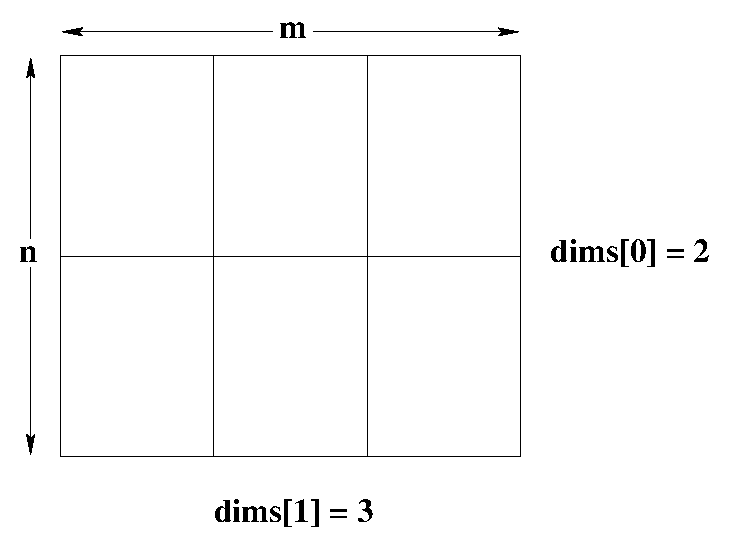
\includegraphics[width=8cm]{Day3/images/topology.eps}
\end{center}
(source : Andrew Siegel, University of Chicago)
\end{frame}


\begin{frame}[containsverbatim]
\frametitle{Virtual topology example}
\begin{lstlisting}[language=C,frame=lines]
gsizes[0] = m; // no. of rows in global array
gsizes[1] = n; // no. of columns in global array
psizes[0] = 2; // no. of procs. in vert. dimension
psizes[1] = 3; // no. of procs. in hori. dimension
lsizes[0] = m/psizes[0]; // no. of rows in local array
lsizes[1] = n/psizes[1]; // no. of columns in local array
dims[0] = 2; dims[1] = 3;
periods[0] = periods[1] = 1;
MPI_Cart_create(MPI_COMM_WORLD, 2, dims, periods, 0, &comm);
MPI_Comm_rank(comm, &rank);
MPI_Cart_coords(comm, rank, 2, coords);
\end{lstlisting}
(source : Andrew Siegel, University of Chicago)
\end{frame}

\begin{frame}[containsverbatim]
\frametitle{Generic virtual topologies}
\begin{itemize}
	\item{Operations on the new \verb+comm+ communicator : get the coordinates}
\end{itemize}

\begin{lstlisting}[language=C,frame=lines]
MPI_Comm_rank(comm, &rank);
MPI_Cart_coords(comm, rank, 2, coords);
printf("Process %d has position (%d, %d) \n", rank, coords[0], coords[1]);
\end{lstlisting}

\begin{itemize}
	\item{get a neighbor rank \verb+int MPI_Cart_shift(MPI_Comm comm,int direction,int displ,int *source,int *dest);+}
\end{itemize}

\begin{lstlisting}[language=C,frame=lines]
MPI_Cart_shift(comm, 0, 1, &prank, &prank_south);
\end{lstlisting}

\end{frame}




\begin{frame}[containsverbatim]
\frametitle{Back to the subarrays}
\begin{lstlisting}[language=C,frame=lines]
start_indices[0] = coords[0] * lsizes[0];
start_indices[1] = coords[1] * lsizes[1];
MPI_Type_create_subarray(2, gsizes, lsizes, start_indices, MPI_ORDER_C, MPI_FLOAT, &filetype);
MPI_Type_commit(&filetype);
MPI_File_open(MPI_COMM_WORLD, "/pfs/datafile", MPI_MODE_CREATE | MPI_MODE_WRONLY, MPI_INFO_NULL, &fh);
MPI_File_set_view(fh, 0, MPI_FLOAT, filetype, "native", MPI_INFO_NULL);
local_array_size = lsizes[0] * lsizes[1];
MPI_File_write_all(fh, local_array, local_array_size, MPI_FLOAT, &status);
\end{lstlisting}
(source : Andrew Siegel, University of Chicago)
\end{frame}

\begin{frame}[containsverbatim]
\frametitle{MPI IO remarks}
\begin{itemize}
	\item {The \verb+I+ versions (non-blocking) exist}
	\item {use collectives as often as possible (except on GPFS file system)}
	\item {contigous / non-contiguous data can lead to tricky implementations}
	\item {MPI IO is efficient on parallel file systems (such as all the clusters at EPFL). It can slow down a code on a simple Desktop/laptop}
\end{itemize}
\end{frame}




\subsection{``v-versions'' of collectives}


\begin{frame}[containsverbatim]
\frametitle{Reminder : Collective communications}

\begin{center}
% Slide 152
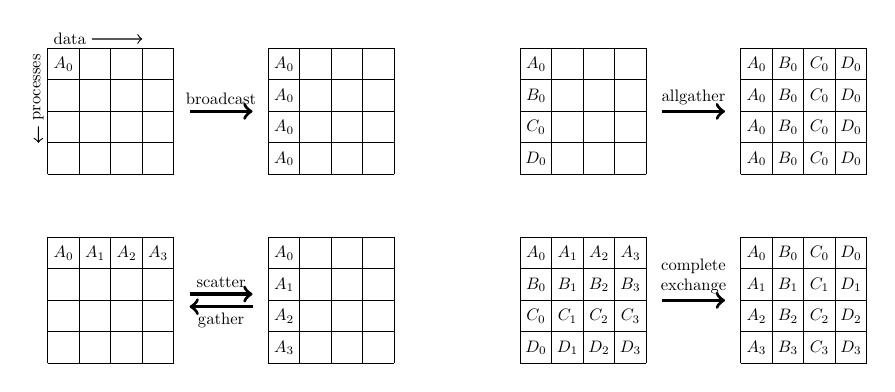
\begin{tikzpicture}[scale = 0.4, every node/.style={scale=0.6}]

\begin{scope}
	\begin{scope}
	\node[anchor = west] (Data) at (0, 4.3) {data};
	\node[anchor = east, rotate = 90] (Proc) at (-0.3, 4) {processes};
	\draw[->] (Data) -- (3, 4.3);
	\draw[->] (Proc) -- (-0.3, 1);
	\draw[step = 1cm] (0,0) grid (4,4);

	\node at (0.5, 3.5) {$A_0$};
	\end{scope}

	\draw[->, very thick] (4.5, 2) -- node[midway, above] {broadcast} (6.5, 2);

	\begin{scope}[xshift = 7cm]
	\draw[step = 1cm] (0,0) grid (4,4);

	\foreach \y in {0.5, 1.5, ..., 3.5}
		\node at (0.5, 4 - \y) {$A_0$};
	\end{scope}

	\begin{scope}[yshift = -6cm]
	\draw[step = 1cm] (0,0) grid (4,4);

	\foreach \x [count = \i from 0] in {0.5, 1.5, ..., 3.5}
		\node at (\x, 3.5) {$A_\i$};
	\end{scope}

	\draw[->, very thick] (4.5, -3.8) -- node[midway, above] {scatter} (6.5, -3.8);
	\draw[<-, very thick] (4.5, -4.2) -- node[midway, below] {gather} (6.5, -4.2);

	\begin{scope}[yshift = -6cm, xshift = 7cm]
	\draw[step = 1cm] (0,0) grid (4,4);

	\foreach \x [count = \i from 0] in {0.5, 1.5, ..., 3.5}
		\node at (0.5, 4 - \x) {$A_\i$};
	\end{scope}
\end{scope}

\begin{scope}[xshift = 15cm]
	\begin{scope}[yshift = 0cm]
	\draw[step = 1cm] (0,0) grid (4,4);

	\foreach \y/\l in {0.5/A, 1.5/B, 2.5/C, 3.5/D}
		\node at (0.5, 4 - \y) {$\l_0$};
	\end{scope}

	\draw[->, very thick] (4.5, 2) -- node[midway, above] {allgather} (6.5, 2);

	\begin{scope}[yshift = 0cm, xshift = 7cm]
	\draw[step = 1cm] (0,0) grid (4,4);

	\foreach \y in {0.5, 1.5, ..., 3.5} {
		\foreach \x/\l in {0.5/A, 1.5/B, 2.5/C, 3.5/D} {
			\node at (\x, 4 - \y) {$\l_0$};
		}
	}
	\end{scope}

	\begin{scope}[yshift = -6cm]
	\draw[step = 1cm] (0,0) grid (4,4);

	\foreach \y/\l in {0.5/A, 1.5/B, 2.5/C, 3.5/D} {
		\foreach \x[count = \i from 0] in {0.5, 1.5, ..., 3.5} {
			\node at (\x, 4 - \y) {$\l_\i$};
		}
	}
	\end{scope}

	\draw[->, very thick] (4.5, -4) -- node[midway, above, align = center] {complete \\ exchange} (6.5, -4);

	\begin{scope}[yshift = -6cm, xshift = 7cm]
	\draw[step = 1cm] (0,0) grid (4,4);

	\foreach \x/\l in {0.5/A, 1.5/B, 2.5/C, 3.5/D} {
		\foreach \y[count = \i from 0] in {0.5, 1.5, ..., 3.5} {
			\node at (\x, 4 - \y) {$\l_\i$};
		}
	}
	\end{scope}
\end{scope}

\end{tikzpicture}

\end{center}

\end{frame}


\begin{frame}[containsverbatim]
\frametitle{``v-version'' of \texttt{MPI$\_$Gather} : \texttt{MPI$\_$Gatherv}}
\begin{itemize}
	\item {adds a stride at receiving ends}
	\item {(example does not work if \texttt{stride > 100})}
\end{itemize}

\begin{center}
% Slide 223
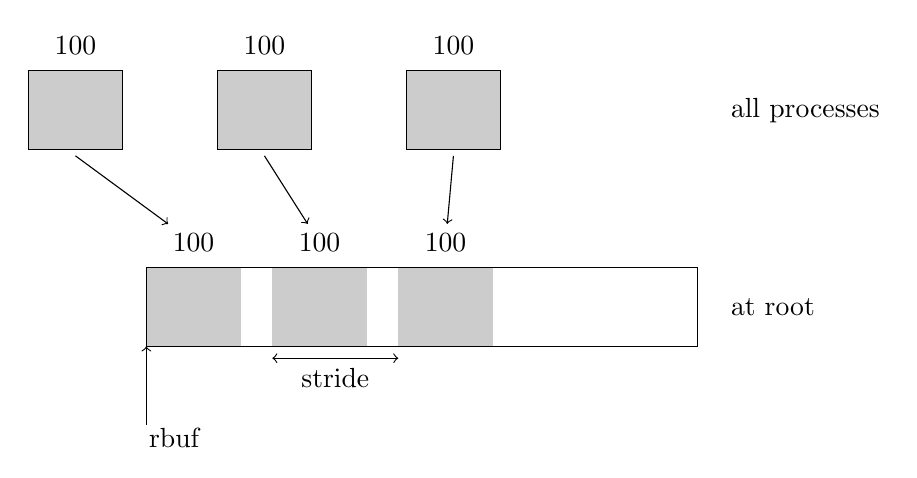
\begin{tikzpicture}

\foreach \x in {0, 1.6, 3.2} {
	\fill[gray!40!white] (\x, 0) rectangle (\x + 1.2, 1);
	\node[anchor = south] (N) at ({(2 * \x + 1.2)/ 2}, 1.08) {100};

	\pgfmathsetmacro{\xtop}{1.5 * (\x - 1)}
	\pgfmathsetmacro{\xmid}{(2 * \xtop + 1.2)/ 2}
	\draw[fill = gray!40!white] ({\xtop}, 2.5) rectangle ({\xtop + 1.2}, 3.5);
	\node[anchor = south] at (\xmid, 3.58) {100};

	\draw[<-] (N) -- (\xmid, 2.42);
}

\draw (0,0) rectangle (7, 1);

\node[anchor = west] at (7.3, 0.5) {at root};
\node[anchor = west] at (7.3, 3) {all processes};

\node[anchor = north west, outer sep = 0pt, inner sep = 1pt] (S) at (0, -1) {rbuf};
\draw[->] (S.north west) -- (0,0);

\draw[<->] (1.6, -0.15) -- node[midway, below] {stride} (3.2, -0.15);

\end{tikzpicture}

\end{center}

\end{frame}


\begin{frame}[containsverbatim]
\frametitle{``v-version'' of \texttt{MPI$\_$Gather} : \texttt{MPI$\_$Gatherv}}
\begin{lstlisting}[language=C,frame=lines]
MPI_Comm comm;
int gsize,sendarray[100];
int root, *rbuf, stride;
int *displs,i,*rcounts;
...
MPI_Comm_size(comm, &gsize);
rbuf = (int *)malloc(gsize*stride*sizeof(int));
displs = (int *)malloc(gsize*sizeof(int));
rcounts = (int *)malloc(gsize*sizeof(int));
for (i=0; i<gsize; ++i) {
   displs[i] = i*stride;
   rcounts[i] = 100;
}
MPI_Gatherv(sendarray, 100, MPI_INT, rbuf, rcounts, displs, MPI_INT,root, comm);
\end{lstlisting}
\end{frame}


\begin{frame}[containsverbatim]
\frametitle{``v-version'' of \texttt{MPI$\_$Scatter} : \texttt{MPI$\_$Scatterv}}
\begin{itemize}
	\item {adds a stride at sending ends}
	\item {(example does not work if \texttt{stride > 100})}
\end{itemize}

\begin{center}
% Slide 223
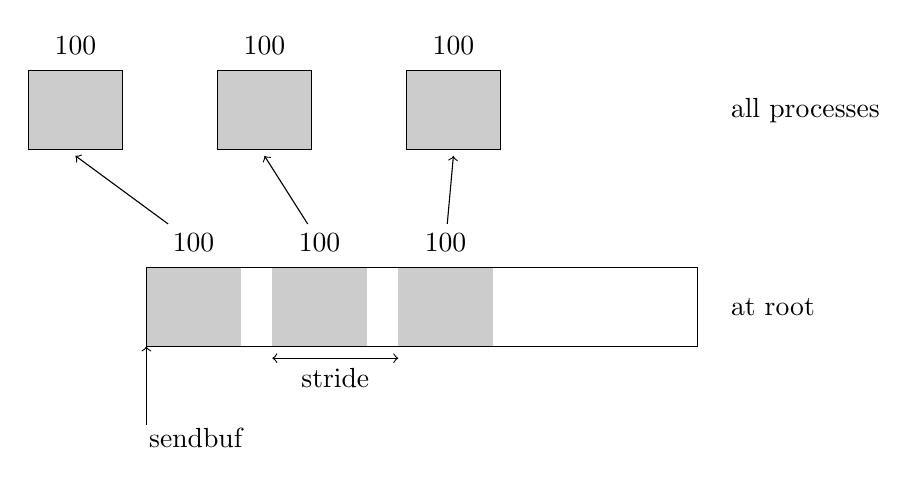
\begin{tikzpicture}

\foreach \x in {0, 1.6, 3.2} {
	\fill[gray!40!white] (\x, 0) rectangle (\x + 1.2, 1);
	\node[anchor = south] (N) at ({(2 * \x + 1.2)/ 2}, 1.08) {100};

	\pgfmathsetmacro{\xtop}{1.5 * (\x - 1)}
	\pgfmathsetmacro{\xmid}{(2 * \xtop + 1.2)/ 2}
	\draw[fill = gray!40!white] ({\xtop}, 2.5) rectangle ({\xtop + 1.2}, 3.5);
	\node[anchor = south] at (\xmid, 3.58) {100};

	\draw[->] (N) -- (\xmid, 2.42);
}

\draw (0,0) rectangle (7, 1);

\node[anchor = west] at (7.3, 0.5) {at root};
\node[anchor = west] at (7.3, 3) {all processes};

\node[anchor = north west, outer sep = 0pt, inner sep = 1pt] (S) at (0, -1) {sendbuf};
\draw[->] (S.north west) -- (0,0);

\draw[<->] (1.6, -0.15) -- node[midway, below] {stride} (3.2, -0.15);

\end{tikzpicture}

\end{center}

\end{frame}


\begin{frame}[containsverbatim]
\frametitle{``v-version'' of \texttt{MPI$\_$Scatter} : \texttt{MPI$\_$Scatterv}}
\begin{lstlisting}[language=C,frame=lines]
MPI_Comm comm;
int gsize,*sendbuf;
int root, rbuf[100], i, *displs, *scounts;
...
MPI_Comm_size(comm, &gsize);
sendbuf = (int *)malloc(gsize*stride*sizeof(int));
...
displs = (int *)malloc(gsize*sizeof(int));
scounts = (int *)malloc(gsize*sizeof(int));
for (i=0; i<gsize; ++i) {
   displs[i] = i*stride;
   scounts[i] = 100;
}
MPI_Scatterv(sendbuf, scounts, displs, MPI_INT, rbuf, 100, MPI_INT, root, comm);
\end{lstlisting}
\end{frame}




\subsection{Non-blocking collectives (NBC)}


\begin{frame}[containsverbatim]
\frametitle{Non-blocking collectives (NBC) for what ?}
\begin{itemize}
	\item{Same situations as for non-blocking point-to-point communications :
		\begin{itemize}
			\item {small message sizes}
			\item {enough computation to perform between start and end of the communication}
			\item {algorithm that authorizes to compute with a partial knowledge of the data}
		\end{itemize}
	}
%	\item{}
\end{itemize}
\end{frame}

\begin{frame}[containsverbatim]
\frametitle{Non-blocking collectives (NBC)}
\begin{itemize}
	\item{\verb+int MPI_Ibarrier(MPI_Comm comm,+\\\verb+MPI_Request *request)+ : NB version of \verb+MPI_Barrier()+}
	\item{\verb+int MPI_Ibcast(void* buffer, int count,+\\\verb+ MPI_Datatype datatype, int root,MPI_Comm comm, MPI_Request *request)+ : NB version of \verb+MPI_Bcast()+. Example :

\begin{lstlisting}[language=C,frame=lines]
MPI_Comm comm;
int array1[100], array2[100];
int root=0;
MPI_Request req;
...
MPI_Ibcast(array1, 100, MPI_INT, root, comm, &req);
compute(array2, 100);
MPI_Wait(&req, MPI_STATUS_IGNORE);
\end{lstlisting}
	}
\end{itemize}
\end{frame}


\begin{frame}[containsverbatim]
\frametitle{Non-blocking collectives (NBC)}
Scatter/Gather versions
\begin{itemize}
	\item{\verb+int MPI_Igather()+ : NB version of \verb+int MPI_Gather()+}
	\item{\verb+int MPI_Igatherv()+ : NB version of \verb+int MPI_Gatherv()+}
	\item{\verb+int MPI_Iscatter()+ : NB version of \verb+int MPI_Scatter()+}
	\item{\verb+int MPI_Iscatterv()+ : NB version of \verb+int MPI_Scatterv()+}
\end{itemize}
All Scatter/Gather versions
\begin{itemize}
	\item{\verb+int MPI_Iallgather()+ : NB version of \verb+int MPI_Allgather()+}
	\item{\verb+int MPI_Iallgatherv()+ : NB version of \verb+int MPI_Allgatherv()+}
\end{itemize}
\end{frame}


\begin{frame}[containsverbatim]
\frametitle{Non-blocking collectives (NBC)}
All to all
\begin{itemize}
	\item{\verb+int MPI_Ialltoall()+ : NB version of \verb+int MPI_Alltoall()+}
	\item{\verb+int MPI_Ialltoallv()+ : NB version of \verb+int MPI_Alltoallv()+}
	\item{\verb+int MPI_Ialltoallw()+ : NB version of \verb+int MPI_Alltoallw()+}
\end{itemize}
\end{frame}

\begin{frame}[containsverbatim]
\frametitle{Non-blocking collectives (NBC)}
Reduce
\begin{itemize}
	\item{\verb+int MPI_Ireduce()+ : NB version of \verb+int MPI_Reduce()+}
	\item{\verb+int MPI_Iallreduce()+ : NB version of \verb+int MPI_Allreduce()+}
	\item{\verb+int MPI_Ireduce_scatter_block()+ : NB version of \verb+int MPI_Reduce_scatter_block()+}
	\item{\verb+int MPI_Ireduce_scatter()+ : NB version of \verb+int MPI_Reduce_scatter()+}
\end{itemize}
Scan
\begin{itemize}
	\item{\verb+int MPI_Iscan()+ : NB version of \verb+int MPI_Scan()+}
	\item{\verb+int MPI_Iexscan+ : NB version of \verb+int MPI_Exscan+}
\end{itemize}
\end{frame}


%\subsection{Virtual topologies}
%
%\begin{frame}[containsverbatim]
%\frametitle{Virtual topology}
%\begin{itemize}
%	\item{The communication pattern of a set of processes can be represented by a graph}
%	\item{nodes are processes, edges are connections}
%	\item{MPI provides functions to create a user defined topology}
%\end{itemize}
%A simple example is the cartesian topology :
%\begin{lstlisting}[language=C,frame=lines]
%int MPI_Cart_create(MPI_Comm comm_old, int ndims, const int dims[], const int periods[], int reorder, MPI_Comm *comm_cart)
%\end{lstlisting}
%\end{frame}


%\begin{frame}[containsverbatim]
%\frametitle{Virtual topology cartesian example}
%\begin{center}
%% Slide 231

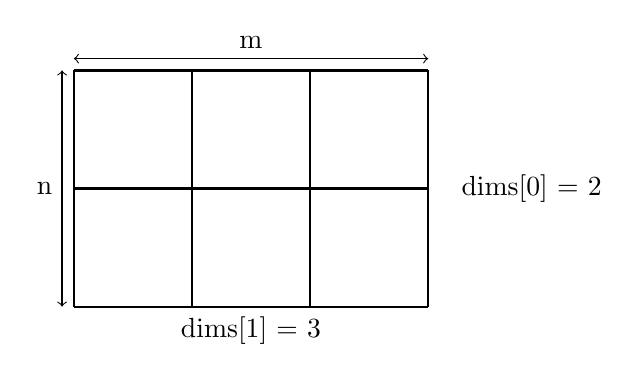
\begin{tikzpicture}

\draw[thick, step = 1.5cm] (0,0) grid (4.5, 3);
\node at (2.25, -0.3) {dims[1] = 3};
\node[anchor = west] at (4.8, 1.5) {dims[0] = 2};

\draw[<->, xshift = -0.15cm] (0,0) -- node[midway, left] {n} (0, 3);
\draw[<->, yshift = 0.15cm] (0,3) -- node[midway, above] {m} (4.5, 3);


\end{tikzpicture}

%\end{center}
%(source : Andrew Siegel, University of Chicago)
%\end{frame}


%\begin{frame}[containsverbatim]
%\frametitle{Virtual topology cartesian example}
%\begin{lstlisting}[language=C,frame=lines]
%gsizes[0] = m; // no. of rows in global array
%gsizes[1] = n; // no. of columns in global array
%psizes[0] = 2; // no. of procs. in vert. dimension
%psizes[1] = 3; // no. of procs. in hori. dimension
%lsizes[0] = m/psizes[0]; // no. of rows in local array
%lsizes[1] = n/psizes[1]; // no. of columns in local array
%dims[0] = 2; dims[1] = 3;
%periods[0] = periods[1] = 1;
%MPI_Cart_create(MPI_COMM_WORLD, 2, dims, periods, 0, &comm);
%\end{lstlisting}
%(source : Andrew Siegel, University of Chicago)
%\end{frame}

%\begin{frame}[containsverbatim]
%\frametitle{Generic virtual topologies}
%\begin{itemize}
%	\item{Operations on the new \verb+comm+ communicator : get the coordinates}
%\end{itemize}

%\begin{lstlisting}[language=C,frame=lines]
%MPI_Comm_rank(comm, &rank);
%MPI_Cart_coords(comm, rank, 2, coords);
%printf("Process %d has position (%d, %d) \n", rank, coords[0], coords[1]);
%\end{lstlisting}

%\begin{itemize}
%	\item{get a neighbor rank \verb+int MPI_Cart_shift(MPI_Comm comm,int direction,int displ,int *source,int *dest);+}
%\end{itemize}
%
%\begin{lstlisting}[language=C,frame=lines]
%MPI_Cart_shift(comm, 0, 1, &prank, &prank_south);
%\end{lstlisting}
%
%\end{frame}


\begin{frame}[containsverbatim]
\frametitle{Generic virtual topologies}
\begin{itemize}
	\item{despite MPI-1 provided functions to create general graph topology (\verb+int MPI_Graph_create()+), it was not scalable (all process needed to know the complete graph)}
	\item{MPI-2.2 introduce the \textit{distributed graph topology} : each process does not need to know the complete graph.}
	\item{\verb+int MPI_Dist_graph_create_adjacent()+ creates a new (local) communicator to which a topology information has been attached. Only adjacent processes. Example : stencil-based algorithm}
	\item{\verb+int MPI_Dist_graph_create()+ : create a new (local) communicator to which a topology has been attached (more general). }
\end{itemize}
\end{frame}

\begin{frame}[containsverbatim]
\frametitle{Generic virtual topologies}
\begin{itemize}
	\item{New collectives are then defined :
		\begin{itemize}
			\item{\verb+int MPI_Neighbor_alltoall+}
			\item{\verb+int MPI_Neighbor_allgather+}
			\item{...}
		\end{itemize}
}
\end{itemize}
\end{frame}


